\documentclass[paper=letter,11pt]{scrartcl}

\KOMAoptions{headinclude=true, footinclude=false}
\KOMAoptions{DIV=14, BCOR=5mm}
\KOMAoptions{numbers=noendperiod}
\KOMAoptions{parskip=half}
\addtokomafont{disposition}{\rmfamily}
\addtokomafont{part}{\LARGE}
\addtokomafont{descriptionlabel}{\rmfamily}
%\setkomafont{pageheadfoot}{\normalsize\sffamily}
\setkomafont{pagehead}{\normalsize\rmfamily}
%\setkomafont{publishers}{\normalsize\rmfamily}
\setkomafont{caption}{\normalfont\small}
\setcapindent{0pt}
\deffootnote[1em]{1em}{1em}{\textsuperscript{\thefootnotemark}\ }


\usepackage{amsmath}
\usepackage[varg]{txfonts}
\usepackage[T1]{fontenc}
\usepackage{graphicx}
\usepackage{xcolor}
\usepackage[american]{babel}
% hyperref is needed in many places, so include it here
\usepackage{hyperref}

\usepackage{xspace}
\usepackage{multirow}
\usepackage{float}


\usepackage{braket}
\usepackage{bbm}
\usepackage{relsize}
\usepackage{tcolorbox}

\def\ketY{\ensuremath{\ket {\Psi}}}
\def\iGeV{\ensuremath{\textrm{GeV}^{-1}}}
%\def\mp{\ensuremath{m_{\textrm{proton}}}}
\def\rp{\ensuremath{r_{\textrm{proton}}}}
\def\me{\ensuremath{m_{\textrm{electron}}}}
\def\aG{\ensuremath{\alpha_G}}
\def\rAtom{\ensuremath{r_{\textrm{atom}}}}
\def\rNucl{\ensuremath{r_{\textrm{nucleus}}}}
\def\GN{\ensuremath{\textrm{G}_\textrm{N}}}
\def\ketX{\ensuremath{\ket{\vec{x}}}}
\def\ve{\ensuremath{\vec{\epsilon}}}


\def\ABCDMatrix{\ensuremath{\begin{pmatrix} A &  B  \\ C  & D \end{pmatrix}}}
\def\xyprime{\ensuremath{\begin{pmatrix} x' \\ y' \end{pmatrix}}}
\def\xyprimeT{\ensuremath{\begin{pmatrix} x' &  y' \end{pmatrix}}}
\def\xy{\ensuremath{\begin{pmatrix} x \\ y \end{pmatrix}}}
\def\xyT{\ensuremath{\begin{pmatrix} x & y \end{pmatrix}}}

\def\IMatrix{\ensuremath{\begin{pmatrix} 0 &  1  \\ -1  & 0 \end{pmatrix}}}
\def\IBoostMatrix{\ensuremath{\begin{pmatrix} 0 &  1  \\ 1  & 0 \end{pmatrix}}}
\def\JThree{\ensuremath{\begin{pmatrix}    0 & -i & 0  \\ i & 0  & 0 \\ 0 & 0 & 0 \end{pmatrix}}} 
\def\JTwo{\ensuremath{\begin{bmatrix}    0 & 0 & -i  \\ 0 & 0  & 0 \\ i & 0 & 0 \end{bmatrix}}}
\def\JOne{\ensuremath{\begin{bmatrix}    0 & 0 & 0  \\ 0 & 0  & -i \\ 0 & i & 0 \end{bmatrix}}}
\def\etamn{\ensuremath{\eta_{\mu\nu}}}
\def\Lmn{\ensuremath{\Lambda^\mu_\nu}}
\def\dmn{\ensuremath{\delta^\mu_\nu}}
\def\wmn{\ensuremath{\omega^\mu_\nu}}
\def\be{\begin{equation*}}
\def\ee{\end{equation*}}
\def\bea{\begin{eqnarray*}}
\def\eea{\end{eqnarray*}}
\def\bi{\begin{itemize}}
\def\ei{\end{itemize}}
\def\fmn{\ensuremath{F_{\mu\nu}}}
\def\fMN{\ensuremath{F^{\mu\nu}}}
\def\bc{\begin{center}}
\def\ec{\end{center}}
\def\nus{$\nu$s}

\def\adagger{\ensuremath{a_{p\sigma}^\dagger}}
\def\lineacross{\noindent\rule{\textwidth}{1pt}}

\newcommand{\multiline}[1] {
\begin{tabular} {|l}
#1
\end{tabular}
}

\newcommand{\multilineNoLine}[1] {
\begin{tabular} {l}
#1
\end{tabular}
}



\newcommand{\lineTwo}[2] {
\begin{tabular} {|l}
#1 \\
#2
\end{tabular}
}

\newcommand{\rmt}[1] {
\textrm{#1}
}


%
% Units
%
\def\m{\ensuremath{\rmt{m}}}
\def\GeV{\ensuremath{\rmt{GeV}}}
\def\pt{\ensuremath{p_\rmt{T}}}


\def\parity{\ensuremath{\mathcal{P}}}

\usepackage{cancel}
\usepackage{ mathrsfs }
\def\bigL{\ensuremath{\mathscr{L}}}

\usepackage{ dsfont }



\usepackage{fancyhdr}
\fancyhf{}


\lhead{\Large 33-444} % \hfill Introduction to Particle Physics \hfill Spring 2022}
\chead{\Large Introduction to Particle Physics} % \hfill Spring 2022}
\rhead{\Large Spring 2022} % \hfill Introduction to Particle Physics \hfill Spring 2022}
\begin{document}
\thispagestyle{fancy}





%\begin{tabular}{c}
%{\large 33-444 \hfill Intro To Particle \hfill Spring 2022\\}
%\hline 
%\end{tabular}

\begin{center}
{\huge \textbf{Final}}
\large

\end{center}

{\large



\textbf{1) What are three major consequences of combining QM and Relativity?}\hfill \textit{(3 points)}\\

\vspace{2.5in}


\textbf{2) Lorentz Transforms } \hfill \textit{(4 points)}\\
\begin{itemize}
\item[a)] How does a \textbf{massive} particle transform under a general Lorentz transformation ($\Lambda_\mu^\nu$) ?\\
eg:  $U(\Lambda] \ket{p^\mu,\sigma} = ?$ 
\vspace*{1in}

\item[b)] How does a \textbf{mass-less} particle $\ket{p^\mu,h}$ transform under a general Lorentz transformation ($\Lambda_\mu^\nu$)?\\
eg:  $U(\Lambda] \ket{p^\mu,h} = ?$ 
\vspace*{1in}

\end{itemize}


\textbf{3) Why do the weak and strong interactions look so different from the electromagnetic interaction despite the fact that at short distances they are all described by similar Feynman diagrams with similar coupling constants?} \hfill \textit{(3 points)}\\


\clearpage

\textbf{4) Lagrangians } \hfill \textit{(3 points)}\\
Consider the following Lagrangian:
\be
L = \frac{1}{2} (\partial_\mu\phi)(\partial^\mu\phi) - \frac{m^2}{2}\phi^2 + \bar{\psi}[i\gamma_\mu\partial^\mu]\psi + g_1 \phi \psi \psi + g_2 \psi \psi \psi \psi + g_3 \phi \phi \phi \phi
\ee

\bi
\item[a)] What is the dimension of $g_1$ ? 
\vspace*{0.5in}
\item[b)] What is the dimension of $g_2$ ? 
\vspace*{0.5in}
\item[c)] What is the dimension of $g_3$ ? 
\vspace*{0.5in}
\ei


\textbf{5) Feynman Diagrams }\hfill \textit{(4 points)}\\
Fermions of type $x$ scatter into fermions of type $y$ through the diagram shown below, where $S$ is a massive scalar. 
At low energies ($P_x P_y << m_S$) the cross section for this process is given by $\sigma_0$.
Assume $m_x$ and $m_y$ are both negligible.
\bc
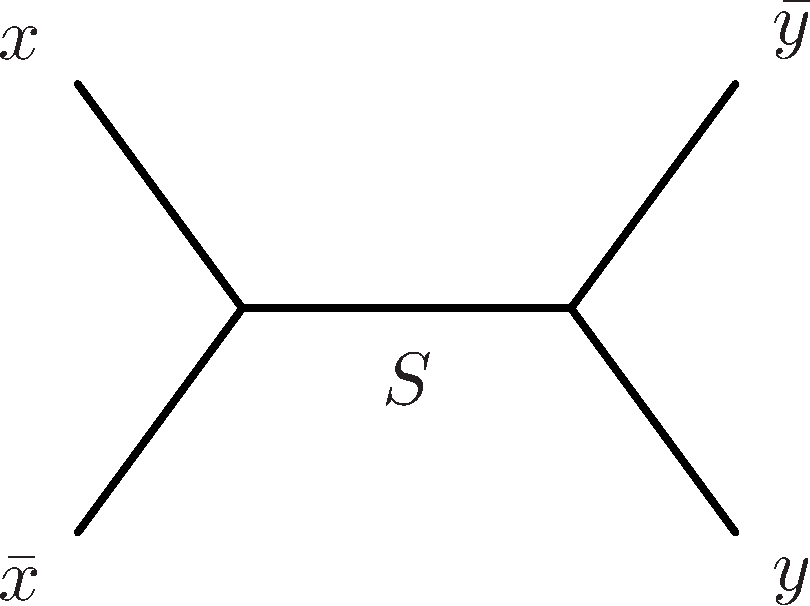
\includegraphics[width=0.2\textwidth]{./xxToyy.pdf}
\ec
\bi
\item[a)] How does this cross section change if the ``S-charge'' of the $x$ particle is doubled ? \\ (S-charge being the $x\bar{x} \rightarrow S$ coupling) 
\vspace*{1.0in}
\item[b)] How does the cross section change if the mass of the $S$-particle is doubled ?
\vspace*{1.0in}
\ei

\clearpage

\textbf{6) Muon decays: } \hfill \textit{(8 points)}\\
\begin{itemize}
  \item[a)]{ The muon decays via the weak interaction.  At low energy ($E << m_W$), this can be approximated as a point-like interaction. 
  Draw the diagram describing muon decay to an electron assuming a point-like weak interaction. 
  \vspace*{1.5in}
}
  \item[b)]{What are the dimensions of the coupling constant, associated to this diagram  ?
\vspace*{1.5in}
  }
  \item[c)] How does the decay rate $\Gamma$ (decays/unit time)  depend on the muon mass ? 
\vspace*{1.5in}
  \item[d)]{ The muon has a mass of $\sim$0.1 GeV and a lifetime of $\sim 1 \mu s$. The tau lepton has a mass of {$\sim$1 GeV}. Estimate the lifetime of the tau lepton in $\mu s$.
\vspace*{1.5in}
}
\end{itemize}

\clearpage


\textbf{7) Branching ratios:  } \hfill \textit{(6 points)}\\
\begin{itemize}
\item[a)]{How often does a $\tau$ decay to a charged lepton ? \\ \textit{(HINT: you can neglect $\tau$ decays to charm and strange quarks) }  
\vspace*{2.0in}
}
\item[b)]{How often does a $Z$-boson decay to charged leptons ?
\vspace*{2.0in}
}
\item[c)]{How often does a $W$-boson decay to a charged lepton ?
\vspace*{2.0in}
}
\end{itemize}


\clearpage

\textbf{8) Electron-positron Collisions } \hfill \textit{(16 points)}\\
\begin{itemize}
\item[a)]{Consider electron-positron collisions with a center-of-mass  energy of 40 GeV.
Estimate the ratio of quark production to di-muon production. 
\vspace*{4.5in}
}
\item[b)]{Sketch a graph of the total cross section of $ee\rightarrow\mu\mu$ as a function of $E_{CM}$ from 40 GeV to 200. 
Also sketch the component of the cross section due to the electro-magnetic interaction.
\vspace*{0.5in}
}
\end{itemize}



\clearpage

\textbf{9) Spontaneous Symmetry Breaking} \hfill \textit{(12 points)} \\ 
\begin{itemize}
\item[a)]{What is Spontaneous Symmetry Breaking  ?  }
\vspace*{1.5in}
\item[b)]{What properties of the fundamental particles is it responsible for describing ?}
\vspace*{1.0in}
\item[c)]{What experimental evidence do we have that spontaneous symmetry breaking is actually responsible for these properties?}
\vspace*{1.0in}
\item[d)]{ What is the particle spectra (ie: for each particle, is it massive or mass-less and what is the spin) from the Lagrangian: \be\mathcal{L} = (\partial_\mu \phi^*) (\partial^\mu \phi) - V(\phi), \textrm{ where } \phi = \phi_1 + i \phi_2,\  V(\phi) = \mu^2\phi^*\phi + \lambda (\phi^*\phi)^2\textrm { and } \lambda, \mu^2 > 0   \ee
\vspace{1.0in}
}
\item[e)]{ What is the particle spectra from the setup in a) but with $\mu^2 < 0$ ?
\vspace{1.0in}
}
\end{itemize}

\clearpage

\textbf{10) Draw one possible Feynman diagram for production and decay of the Higgs boson at the LHC.} \hfill \textit{(4 points)}\\
\vspace{1.5in}

\textbf{11) What is experimental evidence against a fourth generation of leptons ? } \hfill \textit{(4 points)}\\
Other than the fact that they have not be directly observed.
\vspace{1.5in}

\textbf{12) Does the measurement of an electrons energy improve or degrade with increased electron energy? Explain.   } \hfill \textit{(4 points)}\\
\vspace*{1.5in}

\textbf{13) Does the measurement of a muons momentum improve or degrade with increased muon momentum? Explain.   } \hfill \textit{(4 points)}\\


\clearpage

\textbf{14) Beta decay } \hfill \textit{(3 points)}\\
Is $\beta$-decay continuous or discrete ? Why was this question significant ?
\vspace{1.0in}


\textbf{15) Neutrino Physics } \hfill \textit{(10 points)}\\
\begin{itemize}
\item[a)]{How was the distinction between \numu\ and \nue\ discovered ?
\vspace*{1.0in}
}

\item[b)]{Why was the distinction between \numu\ and \nue\  expected ?
\vspace*{1.0in}
}
\item[c)]{What was the main reason to study \nus\ in the 60s and 70s, before we knew they had mass?
\vspace*{0.5in}
}
\item[d)]{What are dominant kind(s) (indicate particle or anti-particle and flavor) of \nus\ that are produced (ignore oscillations) from:
\begin{itemize}
\item[i)]{ The sun ? 
\vspace*{0.25in}
} 
\item[ii)]{Nuclear reactors ? 
\vspace*{0.25in}
}
\item[ii)]{Cosmic-rays ? 
\vspace*{0.25in}
}
\item[iv)]{$\nu$-beams ?
\vspace*{0.25in}
}
\end{itemize}
}
\end{itemize}


\textbf{16) In a two $\nu$ model, what combination of $\Delta m^2$, E, and L do the transition probabilities depend on?  } \hfill \textit{(3 points)}\\
\vspace*{1.5in}

\textbf{17) What was the solar neutrino puzzle ? How was it resolved?  } \hfill \textit{(4 points)}\\
\vspace{1.5in}


\textbf{18) What are the three fundamental length scales in nature and their associated problems.  } \hfill \textit{(6 points)}\\
\vspace{1.0in}


} % Begning Large
\end{document}
